\chapter{Inleiding}

\section{Situering}\label{sec:situering}

UML\cite{RumbaughJames2005Tuml} is een visuele modelleertaal geschikt voor algemene doeleinden. Men gebruikt het om artefacten van een softwaresysteem te specificeren, te visualiseren, te construeren en te documenteren. Deze artefacten bekijken een softwaresysteem vanuit verscheidene oogpunten, en het is de ambitie van UML om genoeg soorten artefacten aan te bieden om een volledige beschrijving te geven van een softwaresysteem. Met behulp van deze artefacten kan men een softwaresysteem ontwerpen, begrijpen, configureren en onderhouden.

Wanneer tijdens het modelleerproces het aantal artefacten toeneemt en als individuele artefacten complex worden, wordt het echter moeilijk om een overzicht te behouden van de structuur van het systeem en hoe de componenten van het systeem zich gedragen. Het kan dat men moeilijk die structuur en dat gedrag begrijpt en dat men tijdens het modelleren beslissingen neemt die ervoor zorgen dat het systeem onmogelijk kan werken als het wordt ge\"implementeerd zoals beschreven in de artefacten of dat het ongewenst gedrag vertoont. Daarom bekijken we in deze masterproef of we voor enkele soorten artefacten, met name klassediagrammen en sequentiediagrammen, gereedschap kunnen aanbieden die de modelleerder helpt om beter inzicht te verkrijgen in wat hij modelleert. Langs de ene kant willen we kijken of de structuur van een klassediagram niet zo is dat het eigenlijk onmogelijk is om te implementeren en of het redundante informatie bevat die het moeilijker maakt om het diagram te begrijpen. Langs de andere kant willen we kijken of we het gedrag beschreven in sequentiediagrammen kunnen simuleren en of we automatisch kunnen controleren of dat gedrag beantwoordt aan bepaalde functionele eisen op het softwaresysteem. We bouwen zulk een gereedschap op door klassediagrammen en sequentiediagrammen te representeren in FO($\cdot$), een uitbreiding van eerste-orde-predicatenlogica.

Sectie \ref{sec:uml-artifacts} geeft een overzicht van de artefacten die UML aanbiedt. Sectie \ref{sec:intro-idp} geeft een inleiding tot IDP\cite{DeCatBroes2014PLaa}, een kennisbanksysteem voor FO($\cdot$). Sectie \ref{sec:research-q} overloopt de probleemstellingen die we bekijken in deze masterproef. Sectie \ref{sec:text-structure} geeft het verdere verloop van deze tekst en beschrijft de bijdragen geleverd in deze masterproef.

\section{Overzicht van UML-artefacten}\label{sec:uml-artifacts}

James Rumbaugh et al.\cite{RumbaughJames2005Tuml} geven een informele indeling van de soorten artefacten in vier domeinen: Het structureel domein, het dynamisch domein, het fysisch domein en het domein van het modelbeheer. De volgende subsecties geven een kort overzicht van elk domein.

\subsection{Structureel domein}

Artefacten in het structureel domein bekijken het softwaresysteem vanuit de volgende oogpunten:

\begin{itemize}
	\item Het statisch oogpunt: Hieronder vallen klassediagrammen. Klasses zijn modelelementen die discrete stukken informatie bevatten in de vorm van attributen. Ze defini\"eren ook bewerkingen die erop uitgevoerd kunnen worden en er wordt ook gespecificeerd met welke andere klasses ze in verband staan door middel van associaties.
	\item Het ontwerpoogpunt: Hieronder vallen interne structuurdiagrammen, collaboratiediagrammen en componentdiagrammen.
	\begin{itemize}
		\item Interne structuurdiagrammen beschrijven voor een bepaalde klasse gedefinieerd in een klassediagram de interne structuur in meer detail.
		\item Collaboratiediagrammen geven weer hoe individuele objecten kunnen samenwerken om een deel van de functionaliteit van de software te bewerkstelligen.
		\item Componentdiagrammen handelen over componenten, welke modulaire delen van een systeem voorstellen die extern zichtbare stukken hebben. Deze extern zichtbare stukken zijn ofwel stukken functionaliteit die de component aanbiedt gelabeld met een naam, genaamd \textit{interfaces}, ofwel een poort gelabeld met de naam van een \textit{interface}, wat betekent dat het component verwacht dat het verbonden wordt met een corresponderende \textit{interface} van een andere component. Componentdiagrammen geven weer hoe componenten met elkaar worden verbonden om op hoog niveau het gedrag van een deel van het systeem te specificeren.
	\end{itemize}
	\item Het \textit{use case} oogpunt: Hieronden vallen \textit{use case} diagrammen. Deze diagrammen benoemen verscheidene actoren, die concrete personen of externe systemen kunnen zijn, en geven grafisch weer welke actoren een rol spelen bij welke \textit{use cases}. De verwachting is dat er elders een tekstuele beschrijving wordt gegeven voor elke \textit{use case}. Een \textit{use case} is een beschrijving van een concrete dienst die een systeem aanbiedt en benoemt de actoren die gebruik willen maken van de dienst, de actoren die betrokken zijn bij het aanleveren van de dienst, en een geordend stappenplan om de dienst aan te leveren.
\end{itemize}

Aangezien deze masterproef onder andere handelt over klassediagrammen, geven we hier een klein voorbeeld. Beschouw volgend klassediagram:

\begin{figure}[H]
	\label{fig:cd}
	\centering
	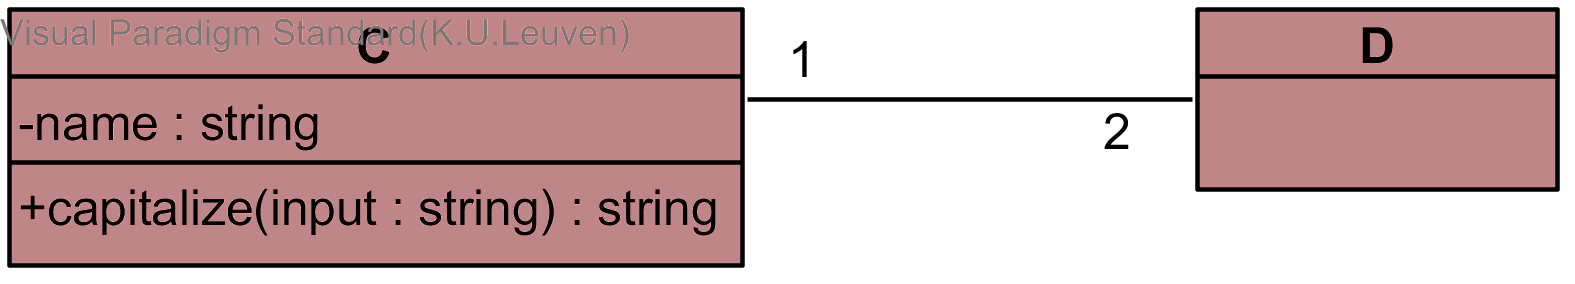
\includegraphics{intro/cd.png}
	\caption{Een voorbeeld van een klassediagram}
\end{figure}

Dit klassediagram drukt uit dat er twee klasses bestaan: \textit{C} en \textit{D}. \textit{C} heeft \'e\'en attribuut, \textit{name}, dat van type \textit{string} is. \textit{D} heeft ook \'e\'en attribuut, \textit{number}, van type \textit{int}. \textit{C} heeft ook \'e\'en operatie \textit{getDNumber} dat \textit{index}, van type \textit{int}, als parameter heeft. \textit{getDNumber(int)} geeft een resultaat terug dat ook van type \textit{int} is. Voorts drukt de lijn tussen \textit{C} en \textit{D} uit dat er een relatie bestaat tussen de twee klasses. Beschouw klasse C. Als we vanuit die klasse de lijn volgen, zien we dat er aan het ander uiteinde staat dat elke \textit{C}-object in relatie moet staan tot exact twee \textit{D}-objecten. Zo ook zien we dat, als we vertrekken vanuit \textit{D}, elk \textit{D}-object in relatie moet staan tot exact \'e\'en \textit{C}-object.

\subsection{Dynamisch domein}

Artefacten in het dynamisch domein bekijken het softwaresysteem vanuit de volgende oogpunten:

\begin{itemize}
	\item Het toestandsautomaatoogpunt: Hieronder vallen toestandsautomaatdiagrammen. Deze diagrammen benoemen toestanden waarin het systeem zich kan bevinden. Deze toestanden worden mogelijks zelf gespecificeerd in een ander toestandsautomaatdiagram. Het diagram beschrijft hoe een systeem van een bepaalde toestand kan overgaan naar een andere toestanden onder bepaalde voorwaarden.
	\item Het activiteitsoogpunt: Hieronder vallen activiteitsdiagrammen. Deze diagrammen beschrijven hoe de besturingsstroom van het systeem kan verlopen tussen activiteiten, welke een voorstelling zijn van een proces dat bestaat binnen het systeem. Men specificeert tussen welke processen het systeem transitioneert onder welke voorwaarden.
	\item Het interactieoogpunt: Hieronder vallen sequentiediagrammen en communicatiediagrammen.
	\begin{itemize}
		\item Sequentiediagrammen beschrijven een tijdverloop van een interactie tussen objecten die instanties zijn van klasses gedefinieerd in een klassediagram. Deze diagrammen beschrijven hoe de toestand van \'e\'en of meerdere objecten verandert ten gevolge van een oproep van een methode gedefinieerd voor de klasse waar een bepaald object een instantie van is. Indien de operatie een resultaat heeft, wordt ook getoond hoe het resultaat wordt berekend.
		\item Communicatiediagrammen zijn gelijkaardig aan sequentiediagrammen, maar in plaats van het tijdverloop centraal te stellen tonen ze expliciet hoe de objecten betrokken in een oproep met elkaar in verband staan. 
	\end{itemize}
\end{itemize}

Aangezien sequentiediagrammen het tweede soort diagram zijn dat we beschouwen in deze masterproef, geven we ook daar een klein voorbeeld van. Beschouw volgend sequentiediagram:

\begin{figure}[H]
	\label{fig:sd}
	\centering
	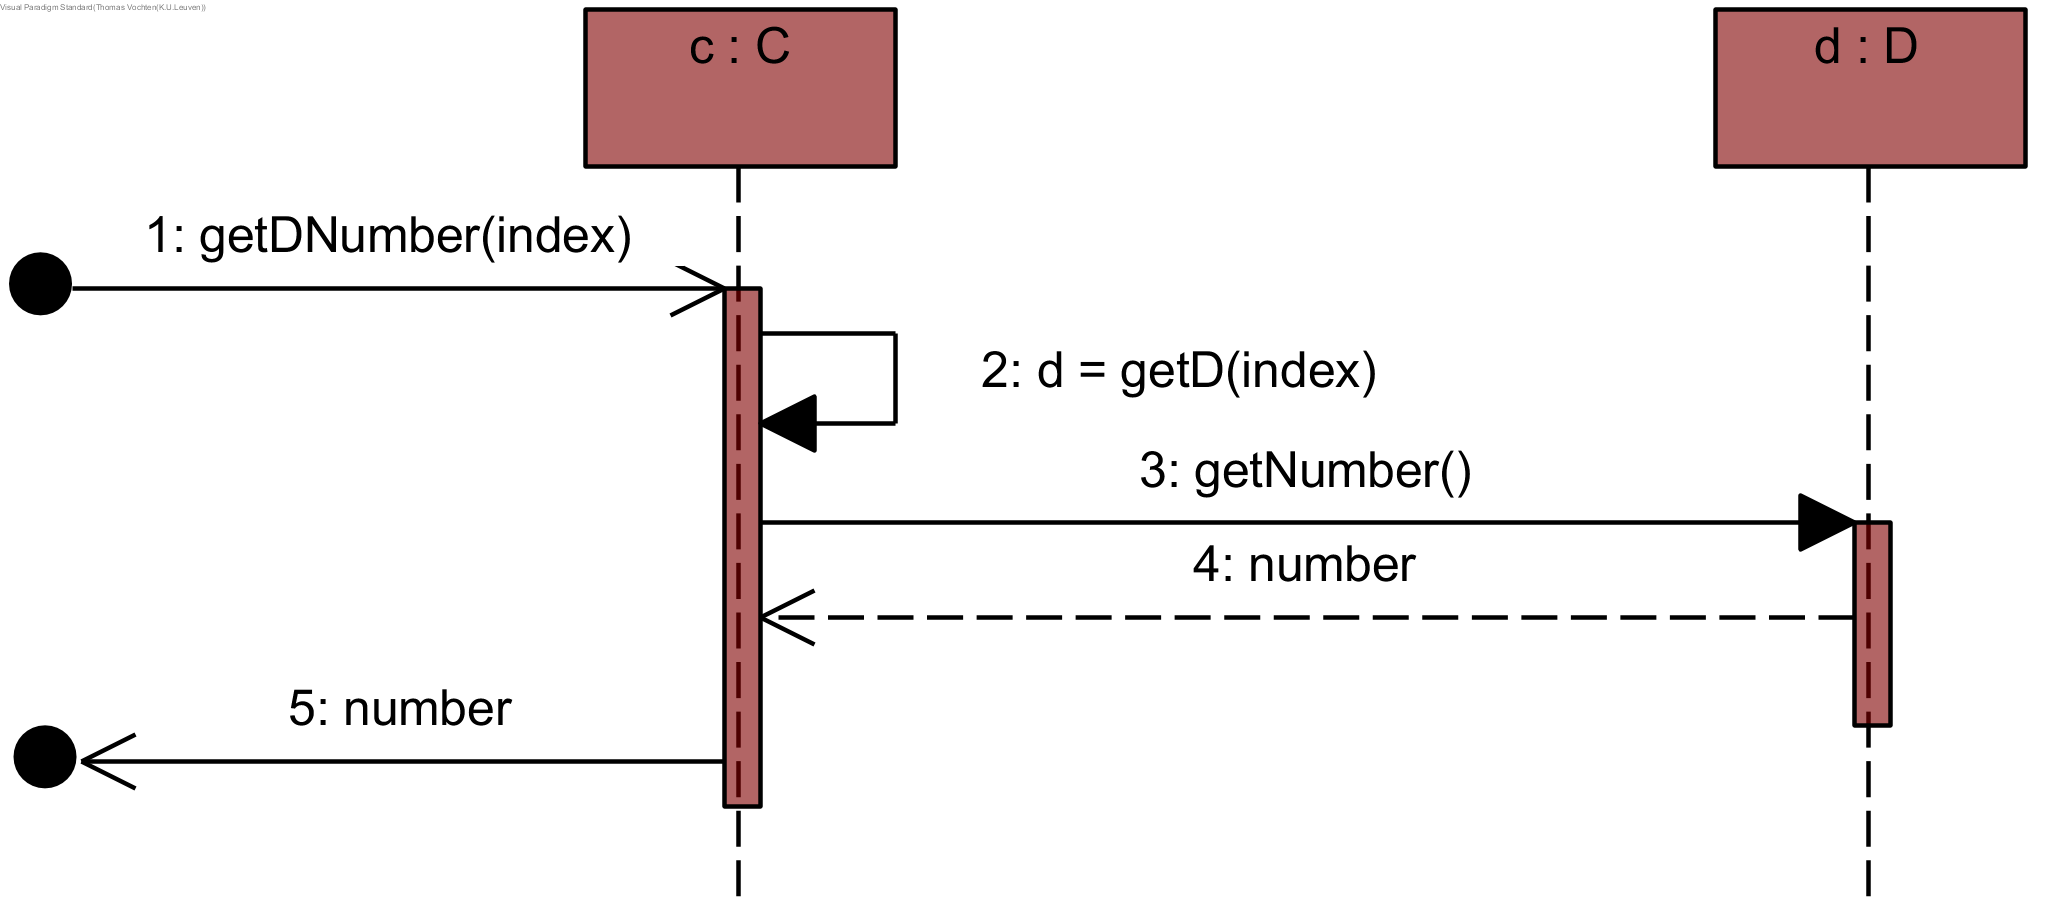
\includegraphics{intro/sd.png}
	\caption{Een voorbeeld van een sequentiediagram}
\end{figure}

Het toont hoe de juiste instantie van \textit{D} wordt opgehaald op basis van invoervariabele \textit{index} en hoe de waarde van het attribuut \textit{number} wordt doorgegeven aan instantie \textit{c}. \textit{c} geeft dan \textit{number} door als uitvoer van het sequentiediagram. Hoofdstuk \ref{sec:gedrag} legt meer in detail uit wat de betekenis is van de elementen die kunnen voorkomen in een sequentiediagram.

\subsection{Fysisch domein}

Artefacten in het fysisch domein bekijken het softwaresysteem vanuit het oogpunt van \textit{deployment}. \textit{Deployment} diagrammen geven weer hoe het systeem fysisch ge\"implementeerd wordt. Deze diagrammen benoemen fysische machines, geven aan welke verbindingen er bestaan tussen die machines en tonen welke concrete softwareartefacten draaien op elke machine.

\subsection{Modelbeheerdomein}

In dit domein beoogt men het beheer van de modellering van het systeem zelf. Tot dit domein behoren de \textit{package} diagrammen. Dit soort diagrammen organiseert de verscheidene soorten modelelementen van het softwaresysteem zoals klasses en \textit{use cases} in \textit{packages}. Een \textit{package} kan ook andere \textit{packages} bevatten. \textit{Package} diagrammen tonen welke \textit{packages} afhankelijk zijn van welke andere \textit{packages}. Zo krijgt men dus een beeld van welke modellen gebruik maken van elementen gedefinieerd in een ander model in hun beschrijving.

\section{Het kennisbanksysteem IDP}\label{sec:intro-idp}

IDP is een kennisbanksysteem\cite{DeCatBroes2014PLaa}. Deze kennisbanken zijn opgesteld in FO($\cdot$), een uitbreiding van predicatenlogica.

IDP bouwt verder op eerder werk in het onderzoeksdomein van het logisch programmeren. Het ondersteunt constructies gebaseerd op logisch programmeren, in het bijzonder inductieve definities, maar breekt ook met enkele fundamentele idee\"en uit dat paradigma. Logische theorie\"en opgesteld in FO($\cdot$) zijn geen uitvoerbare programma's---ze zijn beschrijvingen van mogelijke toestanden in het beschouwde probleemdomein. De fundamentele oplossingsstrategie voor problemen in een toepassingsdomein waar IDP zich op richt is het specificeren van informatie over het domein in logica. De gebruiker past dan een vorm van inferentie toe om een antwoord te krijgen op concrete vragen geformuleerd in termen van het toepassingsdomein.

Bij het opstellen van logische theorie\"en ondersteunt IDP alle concepten uit de klassieke eerste-orde-predicatenlogica: Constanten, variabelen, predicaten, functies en existenti\"ele en universele kwantoren. IDP ondersteunt ook concepten die eerste-orde-predicantelogica uitbreiden. Concreet gaat het over de volgende vier concepten:

\begin{itemize}
	\item \textbf{Logische types}: Alle variabelen gebruikt in een logische zin hebben een type. Dit betekent ook dat alle argumenten van een predicaat en functie en het resultaat van een functie een type hebben.
	\item \textbf{Aggregaten}: Dit zijn de functies \textit{cardinaliteit}, \textit{som}, \textit{product}, \textit{minimum} en \textit{maximum}. De ontwerper specificeert \'e\'en variabele of een tupel van variabelen. Hij bindt die variabele of tupel dan in een logische zin. Als de ontwerper \'e\'en variabele specificeert, worden alle waarden die voldoen aan de logische zin als argument doorgegeven aan de aggregaatfunctie. Als de ontwerper een tupel specificeert, dan wordt voor elke tupel die voldoet aan de zin het eerste element doorgegeven aan de aggregaatfunctie.
	\item \textbf{Inductieve definities}: Dit is een mechanisme om de interpretatie van een predicaat of functie te defini\"eren analoog aan hoe een concept kan gedefinieerd worden in een recursieve definitie in de wiskunde of in verscheidene domeinen van de wetenschap.
	\item \textbf{Parti\"ele functies}: IDP laat toe om een functie te specificeren als \textit{partieel}. Dit betekent dat niet alle elementen van het domein noodzakelijk worden afgebeeld op een element uit het codomein.
\end{itemize}

De inferentievormen die IDP ondersteunt zijn: Modelexpansie gegeven een deels ingevulde structuur; bepalen of een structuur een model is voor een theorie en/of bepalen of een structuur kan uitgebreid worden tot een model voor de theorie; het vinden van optimale modellen gegeven een aggregate term; propagatie, wat gegeven een structuur en een theorie een preciezere structuur geeft die alle oplossingen behoudt; \textit{query}-inferentie, wat alle objecten die beantwoorden aan een bepaalde \textit{query} ophaalt uit een gegeven structuur; deductie; en, gegeven een deels ingevulde structuur en theorie, het berekenen van symmetrische structuren over de theorie.

De basisblokken van een specificatie in IDP zijn als volgt:

\begin{itemize}
	\item \textbf{Vocabularium}: Hier specificeert de ontwerper de logische types die bestaan in het beschouwd domein en de predicaten en functies over die logische types.
	\item \textbf{Theorie}: Hier schrijft de ontwerper zinnen in FO($\cdot$) die bepalen welke structuren over het beschouwde vocabularium modellen zijn. Indien de ontwerper een inconsistente theorie ontwerpt, zullen er geen modellen zijn.
	\item \textbf{Structuur}: De ontwerper vult hier de logische types gedefinieerd in het vocabularium in. \textit{Constructed types} hebben geen invulling nodig aangezien ze al volledig worden gespecificeerd in het vocabularium. De ontwerper kan ook voor \'e\'en of meerdere predicaten aangeven welke tupels wel of geen lid zijn. Hij kan ook voor \'e\'en of meerdere functies specificeren welke elementen uit het domein afgebeeld worden op welk element uit het codomein.
\end{itemize}

De ontwerper kan meerdere vocabularia, theorie\"en en structuren neerschrijven. Elke theorie en structuur kan wel maar de symbolen van \'e\'en vocabularium gebruiken.

Broes De Cat et al.\cite{DeCatBroes2014PLaa} geven een uitgebreidere inleiding tot IDP.

\section{Probleemstellingen}\label{sec:research-q}

Met de mogelijke problemen genoemd in sectie \ref{sec:situering} in het achterhoofd beschouwen we in deze masterproef twee categorie\"en van gebreken in een klassediagram:

\begin{itemize}
	\item \textbf{Inconsistenties:} Het klassediagram is zo opgebouwd dat geen enkele mogelijke toestand van de software kan beantwoorden aan de voorwaarden die worden opgelegd. Dit betekent dat het stuk van de software dat wordt beschreven in het diagram onmogelijk kan werken.
	\item \textbf{Kwaliteitsgebreken:} Deze gebreken hebben een negatieve impact op de kwaliteit van het softwareontwerp. Zo kunnen ze bijvoorbeeld onduidelijkheden in het ontwerp introduceren of het onderhoud van de software \'e\'enmaal ingezet in productie bemoeilijken.
\end{itemize}

We onderzoeken hoe we klassediagrammen kunnen vertalen naar een voorstelling die ons toelaat om automatisch de consistentie van het diagram te controleren en om bepaalde soorten kwaliteitsgebreken op te sporen.

Verder onderzoeken we hoe we sequentiediagrammen kunnen vertalen naar een voorstelling die een uitvoering van het systeem kan simuleren. We kijken ook of we kunnen verifi\"eren of de uitvoer van een sequentiediagram beantwoordt aan de vereisten opgelegd op de methode die dat sequentiediagram modelleert. Het kan immers voorkomen dat een ontwerper een bug introduceert die ervoor zorgt dat uitvoerpaden die verlopen zoals de sequentiediagrammen voorschrijven ongewenste wendingen nemen of zelfs in een oneindige lus terechtkomen. Het kan ook voorkomen dat een sequentiediagram bepaalde controles of bewerkingen mist die ervoor zorgen dat \'e\'en of meerdere eisen ten aanzien van het gedrag van het sequentiediagram niet vervuld zijn.

\section{Verdere verloop van deze tekst}\label{sec:text-structure}

Hoofdstuk \ref{sec:literatuur} geeft een overzicht van literatuur omtrent het gebruik van logica om klassediagrammen en bepaalde soorten dynamische diagrammen voor te stellen.

Hoofdstuk \ref{sec:consistentie} beschrijft hoe we FO($\cdot$) gebruiken om klassediagrammen voor te stellen. We tonen aan dat we consistentie van een klassediagram kunnen verifi\"eren, maar dat er verder onderzoek is vereist om inconsistentie te kunnen controleren.

Hoofdstuk \ref{sec:kwaliteitsgebrek} beschrijft een alternatieve voorstellingswijze die we gebruiken om bepaalde kwaliteitsgebreken op te sporen. We tonen aan dat we de aanwezigheid van losstaande klasses, \textit{many-to-many} associaties en onvoldoende nauw gespecificeerde bovengrenzen op een uiteinde van een associatie kunnen detecteren.

In hoofdstuk \ref{sec:gedrag} beschrijven we hoe sequentiediagrammen voor te stellen in lineaire tijdscalculus\cite{BogaertsBart2014Sdsu}, een methode om in FO($\cdot$) dynamische systemen te modelleren. We geven ook een aanzet om de ontwerptaal beschikbaar voor sequentiediagrammen uit te breiden met declaratieve constructies. Het doel is om ervoor te zorgen dat er significant minder berichten nodig zijn in een sequentiediagram om het gedrag van een methode te specificeren. We gebruiken deze nieuwe constructies om een sequentiediagram te ontwerpen dat het spel Nim modelleert.

In hoofdstuk \ref{sec:evaluatie} evalueren we ons vertalingsproces door een spel te modelleren in een klassediagram en een stel sequentiediagrammen en die diagrammen enerzijds te gebruiken voor een simulatie van het spel en anderzijds om verificaties van gewenste eigenschappen uit te voeren. Daarbij letten we op rekentijd en geheugengebruik. We tonen aan dat we het spel Nim kunnen modelleren in een klassediagram en een stel sequentiediagrammen en dat we met de theorie opgesteld volgens de regels beschreven in hoofdstukken \ref{sec:consistentie} en \ref{sec:gedrag} het verloop van een spel kunnen simuleren. We nemen waar dat er relatief veel tijd en geheugen nodig is om deze simulaties uit te voeren. De resultaten omtrent rekentijd en geheugengebruik duiden we door te vergelijken met een simulatie van het diagram gegeven in hoofdstuk \ref{sec:gedrag} dat gebruik maakt van de nieuwe declaratieve constructies. De conclusie is dat simulatie voor de theorie horend bij dat diagram significant performanter is. Verder tonen we aan dat we kunnen verifi\"eren of de uitvoer van een sequentiediagram voldoet aan bepaalde eisen op de methode gemodelleerd in dat sequentiediagram.

Hoofdstuk \ref{sec:conclusie} geeft een besluit en geeft een aanzet tot verder onderzoek.